\documentclass[11pt,a4paper]{article}

\usepackage[utf8]{inputenc}
\usepackage[T1]{fontenc}
\usepackage[margin=2.4cm]{geometry}
\usepackage{amsmath,amssymb}
\usepackage{booktabs}
\usepackage{tabularx}
\usepackage{enumitem}
\usepackage{xcolor}
\usepackage{tikz}
\usepackage[colorlinks=true,linkcolor=blue!50!black,urlcolor=blue!50!black]{hyperref}
\usetikzlibrary{matrix,positioning,arrows.meta,fit,calc,backgrounds}

\definecolor{nz}{RGB}{38,84,124}
\definecolor{newnz}{RGB}{200,60,50}
\definecolor{ident}{RGB}{60,140,90}
\definecolor{soft}{RGB}{235,240,246}

% Matrix cells: X = nonzero, N = new nonzero (pattern change), O = stored zero, I = identity one, E = empty
\newcommand{\X}{\tikz[baseline=-0.6ex]\fill[nz] (0,0) rectangle (0.26,0.26);}
\newcommand{\N}{\tikz[baseline=-0.6ex]\fill[newnz] (0,0) rectangle (0.26,0.26);}
\renewcommand{\O}{\tikz[baseline=-0.6ex]\draw[nz,line width=0.6pt] (0,0) rectangle (0.26,0.26);}
\newcommand{\I}{\tikz[baseline=-0.6ex]{\fill[ident] (0,0) rectangle (0.26,0.26);\node[white,font=\tiny\bfseries] at (0.13,0.13) {1};}}
\newcommand{\E}{\tikz[baseline=-0.6ex]\path (0,0) rectangle (0.26,0.26);}

\tikzset{
  jac/.style={matrix of nodes, nodes={inner sep=1.2pt, minimum size=0.42cm, anchor=center},
              row sep=0pt, column sep=0pt, left delimiter={[}, right delimiter={]}},
  lab/.style={font=\scriptsize},
  box/.style={draw, rounded corners=2pt, align=center, font=\small, inner sep=5pt, fill=soft},
  arr/.style={-{Stealth[length=2mm]}, line width=0.6pt}
}

\newcommand{\code}[1]{\texttt{\small #1}}
\setlist{itemsep=2pt,topsep=4pt}
\sloppy\emergencystretch=4em
\usepackage{xurl}

\title{One fixed-structure equation system for the CPU and the GPU\\[4pt]
\large Bringing together OLF's alternative equations, the GPU superset matrix\\ and the upstream scatter approach}
\author{olf-gpu design note}
\date{November 2026}

\begin{document}
\maketitle

\begin{abstract}
\noindent Two pieces of work solve the same problem independently. On the CPU, the
\emph{alternative equations} branch of the OLF fork keeps the Jacobian sparsity pattern
constant across PV/PQ switches and contingencies, so that the symbolic factorisation is
built once. On the GPU, this repository builds a \emph{superset} matrix because a uniform
batch requires one pattern for every contingency. A third piece, upstream draft
PR~\href{https://github.com/powsybl/powsybl-open-loadflow/pull/1521}{\#1521}
(``Equation array, scatter approach''), replaces the term-by-term walk of the equation
arrays by precomputed index maps, which is what the GPU kernels already use.

This note describes the three, shows where they agree and where they differ, and proposes
a plan to make OLF own a single fixed-structure description that its own solver runs on
and that the GPU reads as plain arrays instead of re-deriving it.
Nothing in this note has been measured yet; phase~0 of the plan is the measurement.
\end{abstract}

\tableofcontents
\newpage

% =====================================================================================
\section{The problem both sides solve}

OLF's AC equation system has one \emph{column} per active equation and one \emph{row} per
variable. It stores $J^{\mathsf T}$ in compressed-column form; read row by row, the same
arrays are the true Jacobian $J$ in compressed-row form. The figures below show $J$: one
row per equation, one column per variable.

The set of active equations is not constant:
\begin{itemize}
\item a generator reaching a reactive limit replaces its voltage equation by a reactive
      balance (PV$\to$PQ);
\item a contingency removes the equations and variables of the buses it islands, and the
      terms of the branches it opens;
\item a remedial action or a control outer loop adds or removes control equations
      (tap, shunt section, phase shift) together with their variables.
\end{itemize}
Each of these changes the sparsity pattern, the column numbering, or both. On the CPU the
cost is a new symbolic factorisation. On the GPU it is worse: a uniform batch factorises
many matrices in one call and requires them to share one pattern, so a pattern that
depends on the contingency cannot be batched at all.

\paragraph{Running example.} Three buses in a chain, $1 - 2 - 3$. Bus~1 is the slack,
bus~2 holds a generator in voltage control, bus~3 is a load. The variables are
$(\varphi_1, v_1, \varphi_2, v_2, \varphi_3, v_3)$.

\begin{figure}[h]
\centering
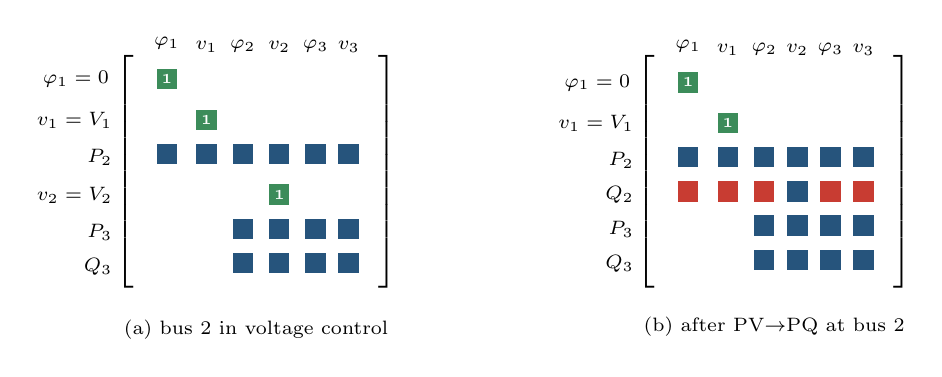
\begin{tikzpicture}
\matrix (A) [jac] {
\I & \E & \E & \E & \E & \E \\
\E & \I & \E & \E & \E & \E \\
\X & \X & \X & \X & \X & \X \\
\E & \E & \E & \I & \E & \E \\
\E & \E & \X & \X & \X & \X \\
\E & \E & \X & \X & \X & \X \\
};
\foreach \r/\t in {1/{$\varphi_1=0$},2/{$v_1=V_1$},3/{$P_2$},4/{$v_2=V_2$},5/{$P_3$},6/{$Q_3$}}
  \node[lab,anchor=east] at ([xshift=-10pt]A-\r-1.west) {\t};
\foreach \c/\t in {1/{$\varphi_1$},2/{$v_1$},3/{$\varphi_2$},4/{$v_2$},5/{$\varphi_3$},6/{$v_3$}}
  \node[lab,anchor=south] at (A-1-\c.north) {\t};
\node[lab,anchor=north] at ([yshift=-6pt]A.south) {(a) bus 2 in voltage control};

\matrix (B) [jac, right=3.6cm of A] {
\I & \E & \E & \E & \E & \E \\
\E & \I & \E & \E & \E & \E \\
\X & \X & \X & \X & \X & \X \\
\N & \N & \N & \X & \N & \N \\
\E & \E & \X & \X & \X & \X \\
\E & \E & \X & \X & \X & \X \\
};
\foreach \r/\t in {1/{$\varphi_1=0$},2/{$v_1=V_1$},3/{$P_2$},4/{$Q_2$},5/{$P_3$},6/{$Q_3$}}
  \node[lab,anchor=east] at ([xshift=-10pt]B-\r-1.west) {\t};
\foreach \c/\t in {1/{$\varphi_1$},2/{$v_1$},3/{$\varphi_2$},4/{$v_2$},5/{$\varphi_3$},6/{$v_3$}}
  \node[lab,anchor=south] at (B-1-\c.north) {\t};
\node[lab,anchor=north] at ([yshift=-6pt]B.south) {(b) after PV$\to$PQ at bus 2};
\end{tikzpicture}
\caption{Legacy modelling. The switch replaces the equation $v_2=V_2$ by $Q_2$ and adds
five nonzeros (red). The pattern changed: the symbolic factorisation is rebuilt.}
\label{fig:legacy}
\end{figure}

% =====================================================================================
\section{Approach A: alternative equations on the CPU}

\paragraph{Where.} OLF fork, branch \code{complementary-equations} (one squashed commit,
July 2026) and its continuation \code{experiment/alt-eq-contingency-fallback}. Opt-in
through the \code{alternativeEquations} parameter of \code{OpenLoadFlowParameters}. Not part of
\code{olf-local-patches}, and 49 commits behind upstream main at the time of writing.

\paragraph{Idea.} An equation owns one matrix column but carries several
\emph{alternative bodies}; exactly one is active. The pattern contributed by the equation
is the union of the patterns of all its alternatives. Entries of the inactive alternatives
are stored as explicit zeros. Switching the active alternative is a value update.

\begin{figure}[h]
\centering
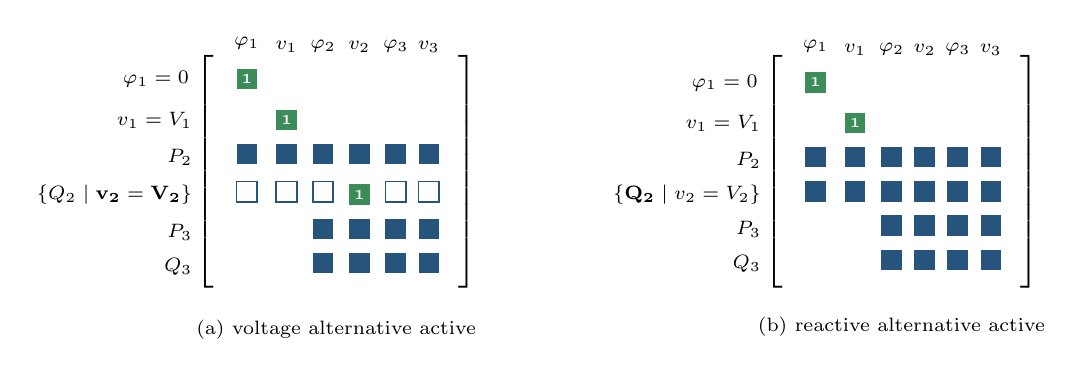
\begin{tikzpicture}
\matrix (A) [jac] {
\I & \E & \E & \E & \E & \E \\
\E & \I & \E & \E & \E & \E \\
\X & \X & \X & \X & \X & \X \\
\O & \O & \O & \I & \O & \O \\
\E & \E & \X & \X & \X & \X \\
\E & \E & \X & \X & \X & \X \\
};
\foreach \r/\t in {1/{$\varphi_1=0$},2/{$v_1=V_1$},3/{$P_2$},4/{$\{Q_2 \mid \mathbf{v_2=V_2}\}$},5/{$P_3$},6/{$Q_3$}}
  \node[lab,anchor=east] at ([xshift=-10pt]A-\r-1.west) {\t};
\foreach \c/\t in {1/{$\varphi_1$},2/{$v_1$},3/{$\varphi_2$},4/{$v_2$},5/{$\varphi_3$},6/{$v_3$}}
  \node[lab,anchor=south] at (A-1-\c.north) {\t};
\node[lab,anchor=north] at ([yshift=-6pt]A.south) {(a) voltage alternative active};

\matrix (B) [jac, right=4.2cm of A] {
\I & \E & \E & \E & \E & \E \\
\E & \I & \E & \E & \E & \E \\
\X & \X & \X & \X & \X & \X \\
\X & \X & \X & \X & \X & \X \\
\E & \E & \X & \X & \X & \X \\
\E & \E & \X & \X & \X & \X \\
};
\foreach \r/\t in {1/{$\varphi_1=0$},2/{$v_1=V_1$},3/{$P_2$},4/{$\{\mathbf{Q_2} \mid v_2=V_2\}$},5/{$P_3$},6/{$Q_3$}}
  \node[lab,anchor=east] at ([xshift=-10pt]B-\r-1.west) {\t};
\foreach \c/\t in {1/{$\varphi_1$},2/{$v_1$},3/{$\varphi_2$},4/{$v_2$},5/{$\varphi_3$},6/{$v_3$}}
  \node[lab,anchor=south] at (B-1-\c.north) {\t};
\node[lab,anchor=north] at ([yshift=-6pt]B.south) {(b) reactive alternative active};
\end{tikzpicture}
\caption{Alternative equations. Hollow squares are stored zeros. Both states share one
pattern, so (a)$\to$(b) changes values only.}
\label{fig:alt}
\end{figure}

\paragraph{What is implemented.}
\begin{itemize}
\item \code{AlternativeEquation} (scalar system) and per-element alternatives inside
      \code{EquationArray} (vectorised system), including an
      \code{elementActiveAlternativeNum[]} array.
\item On the reactive equation of a controller bus: reactive balance, voltage target of
      the controlled bus (local or remote), and reactive distribution (\code{DISTR\_Q})
      when several controllers share the control. The first enabled controller carries
      the voltage target.
\item A \emph{disabled} alternative on $P$ and $Q$ of every eligible bus
      ($\varphi = \text{const}$, $v = \text{const}$), used when a contingency islands the
      bus (figure~\ref{fig:island}).
\item Terms of opened branches stay registered: their entries become stored zeros.
\item A \emph{partial Jacobian update}: after a contingency, restore a snapshot of the
      values and re-derive only the touched columns. The branch's commit notes credit it
      with about a fifth of a large Pegase security analysis.
\end{itemize}

\begin{figure}[h]
\centering
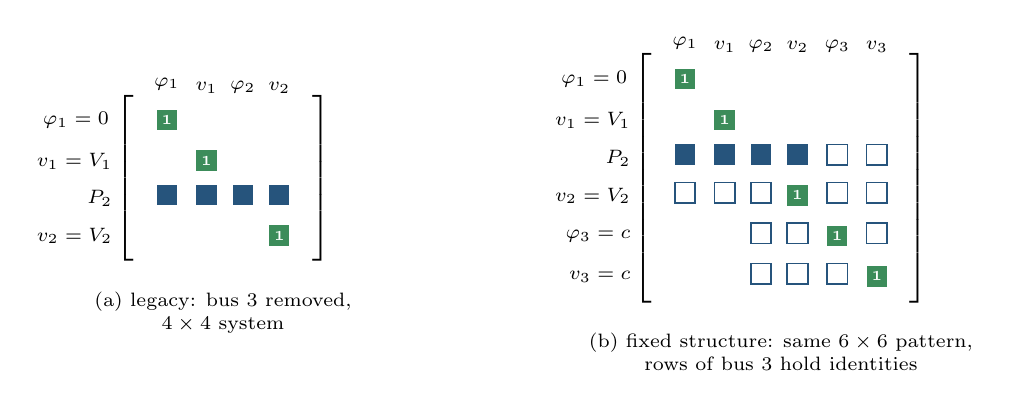
\begin{tikzpicture}
\matrix (A) [jac] {
\I & \E & \E & \E \\
\E & \I & \E & \E \\
\X & \X & \X & \X \\
\E & \E & \E & \I \\
};
\foreach \r/\t in {1/{$\varphi_1=0$},2/{$v_1=V_1$},3/{$P_2$},4/{$v_2=V_2$}}
  \node[lab,anchor=east] at ([xshift=-10pt]A-\r-1.west) {\t};
\foreach \c/\t in {1/{$\varphi_1$},2/{$v_1$},3/{$\varphi_2$},4/{$v_2$}}
  \node[lab,anchor=south] at (A-1-\c.north) {\t};
\node[lab,anchor=north,align=center] at ([yshift=-6pt]A.south) {(a) legacy: bus 3 removed,\\ $4\times4$ system};

\matrix (B) [jac, right=4.4cm of A] {
\I & \E & \E & \E & \E & \E \\
\E & \I & \E & \E & \E & \E \\
\X & \X & \X & \X & \O & \O \\
\O & \O & \O & \I & \O & \O \\
\E & \E & \O & \O & \I & \O \\
\E & \E & \O & \O & \O & \I \\
};
\foreach \r/\t in {1/{$\varphi_1=0$},2/{$v_1=V_1$},3/{$P_2$},4/{$v_2=V_2$},5/{$\varphi_3=c$},6/{$v_3=c$}}
  \node[lab,anchor=east] at ([xshift=-10pt]B-\r-1.west) {\t};
\foreach \c/\t in {1/{$\varphi_1$},2/{$v_1$},3/{$\varphi_2$},4/{$v_2$},5/{$\varphi_3$},6/{$v_3$}}
  \node[lab,anchor=south] at (B-1-\c.north) {\t};
\node[lab,anchor=north,align=center] at ([yshift=-6pt]B.south) {(b) fixed structure: same $6\times6$ pattern,\\ rows of bus 3 hold identities};
\end{tikzpicture}
\caption{Outage of line $2-3$, which islands bus 3.}
\label{fig:island}
\end{figure}

\paragraph{Where it stops.} The following stay on the legacy modelling, either by
eligibility rule or by falling back:
\begin{itemize}
\item buses touching a zero-impedance branch, a converter, or flagged fictitious;
\item buses involved in transformer or shunt voltage control, and the whole run when
      either control is enabled in the parameters;
\item merged or hidden voltage controls, generators with slope, reactive power control;
\item the slack: its angle equation is still a separate equation and its $P$ equation is
      deactivated, so a slack relocation is structural;
\item any solver other than \code{NEWTON\_RAPHSON}, asymmetrical runs, secondary voltage
      control.
\end{itemize}
When a contingency reconfigures a control the alternatives cannot follow, the system is
no longer square. The branch detects this (\code{EquationSystemNotSquareException}) and
re-runs that contingency on a legacy context. Contingencies are reordered so that the
structure-preserving ones run first and share one construction.

% =====================================================================================
\section{Approach B: the fixed superset matrix on the GPU}

\paragraph{Where.} This repository. Rationale in \code{docs/gpu-vs-olf.md} \S1--2;
construction in \path{native/cuda/structure/shared_structure.cu}; host inputs in the
\path{ac/equations/vector/gpu} package and its \code{fixedmatrix} sub-package.

\paragraph{Idea.} The device builds, once, from the base network, the union of everything
any contingency or outer-loop decision may activate. A contingency then changes only
values, per lane of the batch.

\begin{description}
\item[Stable rows.] A row belongs to a \emph{variable}, not to an equation: the $P$ row
      of a bus is the row of its $\varphi$ variable, its $Q$ row the row of its $v$
      variable. Control variables (tap ratio, phase shift, shunt susceptance, the dummy
      variables of a coupler) own a row too. The system is square by construction.
\item[Row mode.] A per-row, per-lane code says which equation the row currently holds
      (\code{GpuRowMode}): \code{FIXED\_VARIABLE} ($x = \text{target}$),
      \code{EQUATION}, \code{BUS\_TARGET\_V\_WITH\_SLOPE}, \code{BRANCH\_TARGET\_P},
      \code{BUS\_TARGET\_Q}, \code{CROSS\_FIXED\_VARIABLE}.
\item[Element mask.] A per-lane mask disables outaged branches, shunts and HVDC links;
      their entries stay in the pattern.
\item[Relocation.] Some equations are written on another variable's row: the voltage
      equation of a transformer-controlled bus sits on the tap row; a remote voltage
      control is carried by one controller's $v$ row, chosen per lane among the
      candidates; a coupler-tree child's balance sits on the coupler's dummy rows. The
      pattern holds the union of all candidate placements.
\item[Role-folded destinations.] For every term output the host precomputes a
      destination: a Jacobian value slot, a mismatch row, or ``skip''. The fill kernels
      only read these arrays.
\end{description}

\begin{figure}[h]
\centering
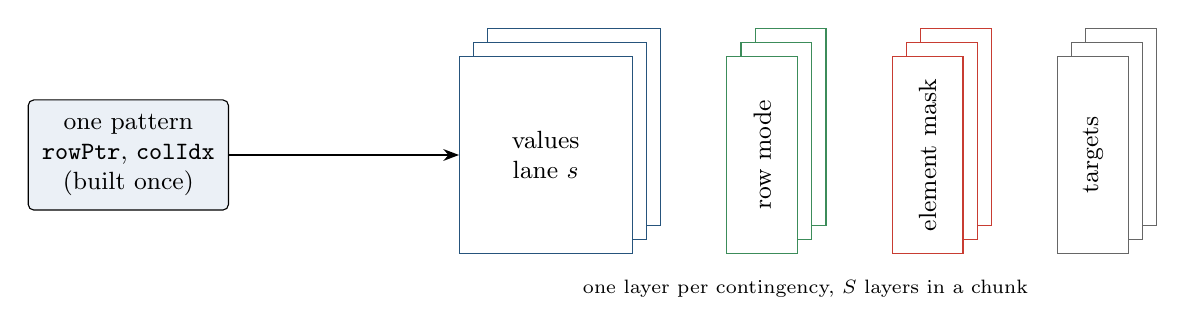
\begin{tikzpicture}[x=1cm,y=1cm]
% pattern
\node[box] (pat) at (0,0) {one pattern\\ \code{rowPtr}, \code{colIdx}\\ (built once)};
% lanes
\foreach \i/\dx/\dy in {3/0.36/0.36,2/0.18/0.18,1/0/0} {
  \draw[fill=white,draw=nz] (4.2+\dx,-1.25+\dy) rectangle (6.4+\dx,1.25+\dy);
}
\node[font=\small,align=center] at (5.3,0) {values\\ lane $s$};
\foreach \i/\dx/\dy in {3/0.36/0.36,2/0.18/0.18,1/0/0} {
  \draw[fill=white,draw=ident] (7.6+\dx,-1.25+\dy) rectangle (8.5+\dx,1.25+\dy);
}
\node[font=\small,align=center,rotate=90] at (8.05,0) {row mode};
\foreach \i/\dx/\dy in {3/0.36/0.36,2/0.18/0.18,1/0/0} {
  \draw[fill=white,draw=newnz] (9.7+\dx,-1.25+\dy) rectangle (10.6+\dx,1.25+\dy);
}
\node[font=\small,align=center,rotate=90] at (10.15,0) {element mask};
\foreach \i/\dx/\dy in {3/0.36/0.36,2/0.18/0.18,1/0/0} {
  \draw[fill=white,draw=black!60] (11.8+\dx,-1.25+\dy) rectangle (12.7+\dx,1.25+\dy);
}
\node[font=\small,align=center,rotate=90] at (12.25,0) {targets};
\draw[arr] (pat.east) -- (4.2,0);
\node[font=\scriptsize] at (8.6,-1.7) {one layer per contingency, $S$ layers in a chunk};
\end{tikzpicture}
\caption{The batched security analysis. The pattern is shared; a contingency is a set of
per-lane arrays.}
\label{fig:batch}
\end{figure}

\paragraph{What it costs today.} The host does not read this structure from OLF: it
re-derives it. The extractor validates OLF's equation system, then rebuilds row
placement, row modes, targets and voltage-control roles from the \code{LfNetwork}, and
the contingency planners mirror OLF's contingency semantics a second time. Rough sizes:
\begin{center}
\begin{tabular}{lr}
\toprule
Layer & Lines \\
\midrule
Java extraction, activation, relocation (\code{vector/gpu}, \code{fixedmatrix}) & $\sim$3\,100 \\
Native pattern construction (\code{structure/}, \code{fixedmatrix/}) & $\sim$3\,400 \\
Java contingency planning that mirrors OLF (\code{batch/plan}) & $\sim$4\,700 \\
\midrule
Whole repository: Java \code{src/main} / native \code{cuda} & 31\,900 / 27\,200 \\
\bottomrule
\end{tabular}
\end{center}
The code comments record the consequence: several bugs came from the mirror disagreeing
with OLF, one of which put 4\,183 of 7\,494 contingencies wrong.

% =====================================================================================
\section{Upstream PR \#1521: the scatter approach}

\paragraph{What it is.} A draft PR by Geoffroy Jamgotchian against upstream main, one
commit, touching \code{EquationArray}, \code{EquationDerivativeVector} and
\code{EquationTermArray} (plus a benchmark). Its description is empty; what follows is
read from the diff.

\paragraph{What it does.} Before, evaluating an equation array \emph{gathered}: for each
equation, walk its terms and fetch each term's value, jumping across the term vectors.
The PR \emph{scatters} instead: read each term vector sequentially and write each value
to a precomputed destination.
\begin{itemize}
\item \code{eval}: per term array, two parallel arrays \code{evalScatterTermElementNums}
      and \code{evalScatterColumns}. Inactive terms and terms of inactive equations are
      filtered out when the arrays are built, so the loop is branch-free.
\item \code{der}: one \code{Scatter} per term derivative vector, mapping
      term element $\to$ position in the flattened derivative vector. Inactive terms
      write zero.
\item The index maps are invalidated whenever activity or numbering changes.
\end{itemize}

\begin{figure}[h]
\centering
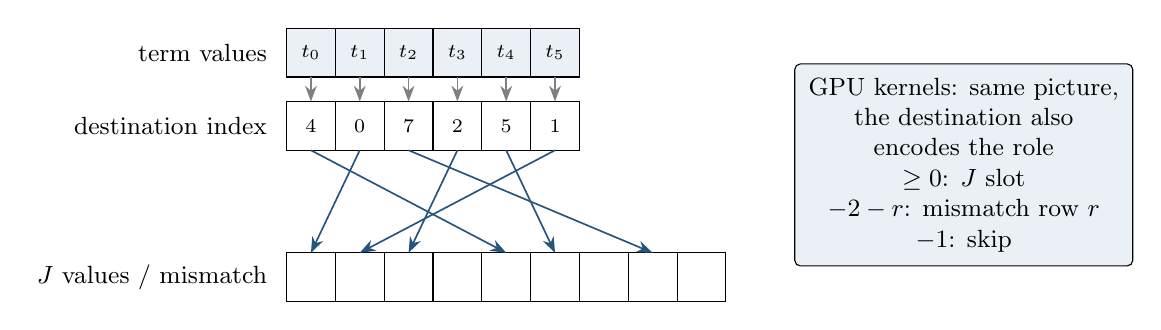
\begin{tikzpicture}[x=0.62cm,y=0.62cm]
% term values
\foreach \i in {0,...,5} { \draw[fill=soft] (\i,3) rectangle (\i+1,4); \node[font=\scriptsize] at (\i+0.5,3.5) {$t_{\i}$}; }
\node[font=\small,anchor=east] at (-0.2,3.5) {term values};
% index
\foreach \i/\d in {0/4,1/0,2/7,3/2,4/5,5/1} { \draw (\i,1.5) rectangle (\i+1,2.5); \node[font=\scriptsize] at (\i+0.5,2) {\d}; }
\node[font=\small,anchor=east] at (-0.2,2) {destination index};
% output
\foreach \i in {0,...,8} { \draw[fill=white] (\i,-1.6) rectangle (\i+1,-0.6); }
\node[font=\small,anchor=east] at (-0.2,-1.1) {$J$ values / mismatch};
\foreach \i/\d in {0/4,1/0,2/7,3/2,4/5,5/1} { \draw[arr,nz] (\i+0.5,1.5) -- (\d+0.5,-0.6); }
\foreach \i in {0,...,5} { \draw[arr,black!50] (\i+0.5,3) -- (\i+0.5,2.5); }
% GPU side
\node[box,anchor=west] at (10.4,1.2) {GPU kernels: same picture,\\ the destination also\\ encodes the role\\ $\geq 0$: $J$ slot\\ $-2-r$: mismatch row $r$\\ $-1$: skip};
\end{tikzpicture}
\caption{Scatter. The CPU PR and the GPU fill kernels use the same data structure: a
destination index per term output.}
\label{fig:scatter}
\end{figure}

\paragraph{Why it matters here.} It is the third leg of the same design.
\begin{itemize}
\item The PR's scatter arrays and the GPU's role-folded destination arrays describe the
      same mapping. If OLF owns the map, the GPU no longer has to rebuild it from the
      generated scatter tables and its own row placement.
\item The PR's weak point is invalidation: every activation change rebuilds the
      \code{eval} maps. Under a fixed structure nothing is ever filtered out, so the maps
      are built once per network and never invalidated. Alternative equations make the
      scatter approach cheaper, and the scatter approach gives alternative equations
      their natural storage.
\item The PR's \code{der} scatter stops at the flattened derivative vector; the last hop
      to the matrix value array still goes through a handler call per entry. Composing
      the two gives a direct ``term derivative $\to$ Jacobian value index'' array, which
      is exactly what a device needs.
\end{itemize}

% =====================================================================================
\section{Side by side}

\begin{center}
\small
\begin{tabularx}{\textwidth}{>{\raggedright\arraybackslash}p{3.1cm}>{\raggedright\arraybackslash}X>{\raggedright\arraybackslash}X}
\toprule
 & CPU alternative equations & GPU superset matrix \\
\midrule
Fixed pattern & union of all alternatives & union of every placement any lane may use \\
Slot identity & a \emph{primary equation} owns a column & a \emph{variable} owns a row \\
Current content of a slot & active alternative & row mode \\
PV$\to$PQ & switch to the reactive alternative & \code{FIXED\_VARIABLE} $\to$ \code{BUS\_TARGET\_Q} \\
Islanded bus & disabled alternative & \code{FIXED\_VARIABLE} in that lane \\
Remote voltage control & first enabled controller carries the target, others \code{DISTR\_Q} & carrier row chosen per lane, \code{DISTR\_Q} pack \\
Branch outage & term inactive, variables kept & element mask \\
Slack & legacy (separate equation) & \code{FIXED\_VARIABLE} on the $\varphi$ row, relocatable \\
Transformer / shunt voltage control & excluded; run falls back & relocation to the tap / susceptance row \\
Zero-impedance branches & excluded & dummy rows, per-lane spanning tree \\
State of a contingency & events mutating one live system & plain arrays per lane \\
When it cannot cope & re-run on a legacy context & send the contingency to the CPU \\
Fill & term walk (scatter with \#1521) & scatter through destination arrays \\
\bottomrule
\end{tabularx}
\end{center}

\paragraph{The three real differences.}
\begin{enumerate}
\item \textbf{Slot identity.} Attaching a column to an equation is what makes the CPU
      branch fragile: control equations and control variables appear and disappear
      together, and a missed case leaves the system non-square. Attaching the slot to
      the variable makes squareness structural. Every GPU ``relocation'' is then simply
      an alternative of the slot of the variable whose row hosts it.
\item \textbf{Coverage.} The GPU already handles, inside the fixed structure, every case
      the CPU branch excludes. \code{docs/gpu-vs-olf.md} \S2 is, in effect, the
      specification of a complete alternative-equations model.
\item \textbf{Mutation versus data.} The CPU applies a contingency to the
      \code{LfNetwork} and lets events update the equation system. The GPU needs the
      contingency as data, for many contingencies at once. A shared description of a
      contingency must therefore be computable without applying it.
\end{enumerate}

% =====================================================================================
\section{Target design}

\begin{figure}[h]
\centering
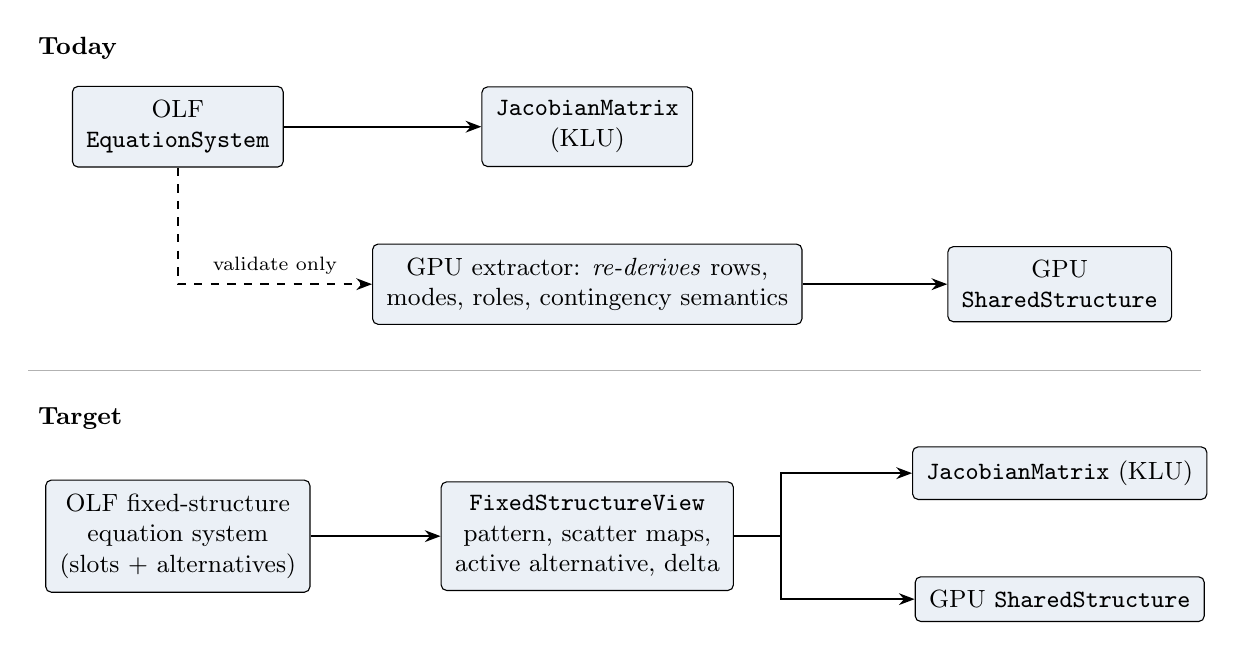
\begin{tikzpicture}[x=1cm,y=1cm]
% today
\node[font=\small\bfseries,anchor=west] at (-1.9,1.0) {Today};
\node[box] (es) at (0,0) {OLF\\ \code{EquationSystem}};
\node[box] (jm) at (5.2,0) {\code{JacobianMatrix}\\ (KLU)};
\node[box] (ex) at (5.2,-2.0) {GPU extractor: \emph{re-derives} rows,\\ modes, roles, contingency semantics};
\node[box] (ss) at (11.2,-2.0) {GPU\\ \code{SharedStructure}};
\draw[arr] (es) -- (jm);
\draw[arr,dashed] (es) |- node[pos=0.75,above,font=\scriptsize]{validate only} (ex);
\draw[arr] (ex) -- (ss);
\draw[black!30] (-1.9,-3.1) -- (13.0,-3.1);
% target
\node[font=\small\bfseries,anchor=west] at (-1.9,-3.7) {Target};
\node[box] (es2) at (0,-5.2) {OLF fixed-structure\\ equation system\\ (slots + alternatives)};
\node[box] (view) at (5.2,-5.2) {\code{FixedStructureView}\\ pattern, scatter maps,\\ active alternative, delta};
\node[box] (jm2) at (11.2,-4.4) {\code{JacobianMatrix} (KLU)};
\node[box] (ss2) at (11.2,-6.0) {GPU \code{SharedStructure}};
\draw[arr] (es2) -- (view);
\draw[arr] (view.east) -- ++(0.6,0) |- (jm2.west);
\draw[arr] (view.east) -- ++(0.6,0) |- (ss2.west);
\end{tikzpicture}
\caption{Today the GPU rebuilds what OLF knows. In the target, both solvers read one
description.}
\label{fig:arch}
\end{figure}

\subsection{Slots owned by variables}

Every variable to solve owns exactly one slot. A slot has an ordered list of
alternatives and one active alternative. Proposed alternatives per variable type:

\begin{center}
\small
\begin{tabularx}{\textwidth}{>{\raggedright\arraybackslash}p{2.6cm}>{\raggedright\arraybackslash}X}
\toprule
Variable & Alternatives of its slot \\
\midrule
\code{BUS\_PHI} & active balance $P$; $\varphi = \text{const}$ (slack, reference, disabled or islanded bus); slack distribution among several slacks \\
\code{BUS\_V} & reactive balance $Q$; local voltage target; voltage target with slope; voltage target of a remote controlled bus; \code{DISTR\_Q}; $v = \text{const}$ (disabled bus) \\
\code{BRANCH\_RHO1} & tap fixed; voltage target of the controlled bus; \code{DISTR\_RHO}; reactive balance of the controlled bus \\
\code{SHUNT\_B} & susceptance fixed; voltage target of the controlled bus; \code{DISTR\_SHUNT\_B} \\
\code{BRANCH\_ALPHA1} & phase shift fixed; \code{BRANCH\_TARGET\_P} of the controlled branch \\
\code{DUMMY\_P}, \code{DUMMY\_Q} & dummy fixed (coupler open or off the tree); \code{ZERO\_PHI} / \code{ZERO\_V}; the relocated balance of a coupler-tree child \\
\bottomrule
\end{tabularx}
\end{center}

The list is the GPU's current row placement rules written as alternatives. Whether every
relocation the GPU performs can be expressed this way is the main thing phase~2 must
prove; the cross identity (\code{CROSS\_FIXED\_VARIABLE}) and the zero-diagonal repair
are the cases to look at first, since they exist for factorisation without pivoting
rather than for modelling.

\subsection{The read-only contract}

OLF exposes one immutable description per equation system, plus a small mutable state:

\begin{description}
\item[Numbering.] Slot index $=$ variable row. Stable for the life of the system.
\item[Pattern.] \code{rowPtr[]}, \code{colIdx[]}: the union pattern. OLF's own sparse
      matrix uses the same arrays.
\item[Alternatives.] Per slot: the list of alternative types, the element each one
      targets (for the target vector), and the range of its entries in the pattern.
\item[Scatter maps.] Per term array and per output (value, each derivative): the
      destination index, as in \#1521 but composed down to the Jacobian value index and
      the mismatch row, and tagged with the alternative it belongs to.
\item[State.] \code{activeAlternative[slot]} and \code{elementActive[element]}. These
      two arrays are the only things a PV/PQ switch or a contingency changes.
\item[Delta.] A contingency or action expressed as a list of changes to the state arrays
      and to the targets, computed from a \code{PropagatedContingency} without applying
      it to the network.
\end{description}

The CPU solver fills its matrix from the scatter maps and the state arrays. The GPU
uploads the pattern and the maps once, and one state array per lane.

\subsection{What stays GPU-specific}

\begin{itemize}
\item The physics: already single-sourced by \code{java2cuda}.
\item Everything needed to factorise without pivoting: the row permutation that pairs
      each row with a dominant diagonal, the zero-diagonal repair, the cross identity,
      adaptive refinement. They become data \emph{derived from} the shared pattern.
\item The device outer loops and the batched solver.
\item Packing of physical parameters (pi-model values, limits). It could later read the
      term arrays' own parameter vectors; that is a separate step.
\end{itemize}

% =====================================================================================
\section{Plan}

Each phase ends on something measurable, and the first three have value for the CPU
alone, which is what makes them proposable upstream. Durations are rough estimates.

\subsection*{Phase 0 --- Measure the gap \hfill (1--2 weeks)}
\begin{enumerate}
\item Rebase the alternative-equations commits onto the current \code{olf-local-patches}.
\item Lift the \code{NEWTON\_RAPHSON}-only gate behind a test-only switch so the GPU
      solver can run on an alternative-equations system.
\item Write a pattern comparison tool: build the CPU union pattern and the GPU superset
      for the same network, map both to variable-row numbering, report the entries in
      one and not the other, by cause.
\item Run it on the IEEE cases, pegase9241 and rte6515.
\item Census: how many buses and controls are ineligible on each network, by rule; how
      many contingencies fall back on the CPU side; how many go to the CPU on the GPU
      side.
\item Measure the cost of the stored zeros on the CPU: KLU fill and factorisation time
      with the GPU superset pattern against the legacy pattern.
\end{enumerate}
\textbf{Exit.} A table of the pattern difference and of the coverage gap, and a go/no-go
on CPU performance. Everything after depends on these numbers.

\subsection*{Phase 1 --- Scatter as the storage \hfill (2--3 weeks)}
\begin{enumerate}
\item Bring \#1521 into the fork (or build on it once merged upstream).
\item Add the composed map ``term derivative $\to$ Jacobian value index''.
\item Under alternative equations, stop filtering inactive terms out of the maps: keep
      them, and let the state arrays decide the value. The maps are then never
      invalidated.
\item Rewrite the partial Jacobian update on top of the maps (re-scatter the entries of
      the touched slots).
\end{enumerate}
\textbf{Exit.} Values and derivatives bit-identical to the current implementation on the
OLF test suite; the PR's own benchmark not slower; no map rebuild during a security
analysis on an eligible network.

\subsection*{Phase 2 --- Variable-owned slots in OLF \hfill (6--10 weeks)}
One sub-step per family, each removing one exclusion, each validated against the legacy
modelling on the whole OLF test suite:
\begin{enumerate}
\item Introduce the slot abstraction; move the existing alternatives (reactive balance,
      voltage target, \code{DISTR\_Q}, disabled bus) onto it. No behaviour change.
\item Slack and reference bus as alternatives of the $\varphi$ slot; slack relocation
      becomes a value change.
\item Generators with slope; merged and hidden voltage controls.
\item Transformer voltage control and shunt voltage control, on the tap and susceptance
      slots.
\item Phase control on the phase-shift slot.
\item Zero-impedance branches: dummy slots, spanning-tree re-election as an alternative
      switch. This is the hardest step; the earlier attempt on the fork was reverted.
\item Converters and fictitious buses, or a documented decision to leave them out.
\end{enumerate}
\textbf{Exit.} On rte6515 with the production parameters, a security analysis performs
one structure build and no non-square fallback; results equal the legacy modelling
within the solver tolerance.

\subsection*{Phase 3 --- The contract \hfill (2--3 weeks)}
\begin{enumerate}
\item Define \code{FixedStructureView} in OLF with the arrays of the previous section.
\item Make \code{JacobianMatrix} fill from it, so the CPU solver is its first consumer.
\item Property test: the matrix assembled from the view equals the matrix assembled by
      the term walk, for random states and random alternative selections.
\end{enumerate}
\textbf{Exit.} The CPU load flow and security analysis run on the view only.

\subsection*{Phase 4 --- The GPU reads the contract \hfill (4--6 weeks)}
\begin{enumerate}
\item Import path: build \code{SharedStructure} from the view's pattern and maps.
\item Run both paths side by side and assert equality of pattern, destinations, row
      modes and targets on every test network. This is the gate.
\item Switch the default; keep the old extractor behind a switch for one release.
\item Delete \code{StableRowIndexing}, \code{ExtractionColumns}, the activation
      extractor, the relocation tables and the native pattern collection.
\end{enumerate}
\textbf{Exit.} The GPU test suite passes with the old extraction removed;
\code{GpuAcValidation} shrinks to a version check on the contract.

\subsection*{Phase 5 --- Contingencies as data \hfill (6--8 weeks)}
\begin{enumerate}
\item Compute the delta of a contingency in OLF without mutating the network.
\item CPU security analysis applies and undoes deltas instead of applying and restoring
      network state; this subsumes the ``restore only impacted elements'' work.
\item The GPU planner packs deltas into lanes; the mirrors in \code{batch/plan} are
      removed family by family (branch outage first, then injections, then voltage
      control re-merge).
\end{enumerate}
\textbf{Exit.} The reject reasons that exist only because the mirror cannot express a
case are gone; remaining rejects are genuine device limits.

\subsection*{Phase 6 --- Upstream}
Propose in this order, each standing on its own: the scatter extensions (after \#1521),
the slot abstraction with the existing alternatives, then one PR per family of phase~2,
then the view. The GPU repository keeps working against the fork until each lands.

\begin{figure}[h]
\centering
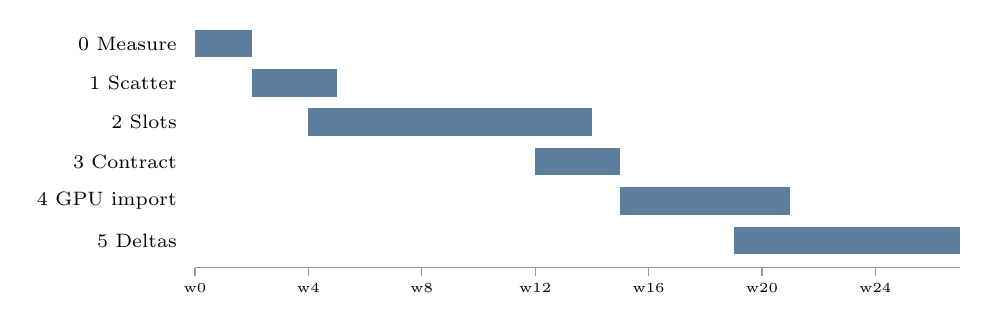
\begin{tikzpicture}[x=0.36cm,y=0.5cm]
\foreach \y/\a/\b/\t in {6/0/2/{0 Measure},5/2/5/{1 Scatter},4/4/14/{2 Slots},3/12/15/{3 Contract},2/15/21/{4 GPU import},1/19/27/{5 Deltas}} {
  \fill[nz!75] (\a,\y-0.35) rectangle (\b,\y+0.35);
  \node[font=\scriptsize,anchor=east] at (-0.3,\y) {\t};
}
\draw[black!40] (0,0.3) -- (27,0.3);
\foreach \x in {0,4,...,24} { \draw[black!40] (\x,0.3) -- (\x,0.1); \node[font=\tiny] at (\x,-0.2) {w\x}; }
\end{tikzpicture}
\caption{Indicative sequencing. Phases 1 and 2 overlap; phase 5 can start once the GPU
reads the contract.}
\end{figure}

% =====================================================================================
\section{Risks and open questions}

\begin{description}
\item[CPU cost of the union pattern.] Stored zeros increase fill. The GPU already pays
      it; whether KLU gains more from one symbolic factorisation than it loses to fill is
      unmeasured (phase~0). \code{DISTR\_Q} on large controller groups and the union of
      carrier candidates are the entries to watch.
\item[Upstream acceptance.] Without it, the maintenance burden moves from this
      repository to the fork rather than disappearing. The alternative-equations change
      is already about 3\,700 lines in OLF's core \code{equations} package. The argument
      is the CPU gain; it has to be demonstrated first.
\item[Zero-impedance spanning tree.] OLF's tree depends on the history of contingencies;
      the GPU replays it. A stateless rule would be simpler for both sides but changes
      OLF behaviour.
\item[Relocations that exist for numerics.] The cross identity and the zero-diagonal
      repair serve factorisation without pivoting. They may belong on the GPU side as
      derived data rather than in the shared model.
\item[Relation to \#1521.] It is a draft with no description; its direction may change.
      Phase~1 should be discussed with its author before building on it.
\item[Incremental LU.] The branch's notes say incremental LU updates on alternative
      switches were benchmarked and did not pay. Not revisited here.
\item[Scope of a first upstream proposal.] The smallest useful unit is probably the slot
      abstraction with today's alternatives and the partial update, on eligible networks
      only.
\end{description}

\section*{References}
\begin{itemize}
\item OLF fork: branches \code{complementary-equations},
      \code{alternative-equations-and-sa-mt-copy},
      \code{experiment/alt-eq-contingency-fallback}.
\item Upstream draft PR \#1521, ``Equation array, scatter approach'':
      \url{https://github.com/powsybl/powsybl-open-loadflow/pull/1521}.
\item This repository: \code{docs/gpu-vs-olf.md} (\S1 one fixed matrix, \S2 stable rows,
      row state, placement, factorisation without pivoting);
      \code{docs/hybrid-outer-loop-production-design.md} \S11;
      \code{native/cuda/structure/shared\_structure.cu}.
\end{itemize}

\end{document}
